\documentclass[a4paper, 12pt]{article}

\usepackage{cmap} % поиск в PDF
\usepackage[english, russian]{babel} % локализация и переносы
\parskip=3pt % дополнительное расстояние между абзацами
\usepackage{graphicx} % вставка рисунков
\usepackage{lastpage}
\usepackage{rotating}
\usepackage{minted} % красивый код
\usepackage{verbatim}
\usepackage{multirow} % Слияние строк в таблице
\usepackage{caption}
\usepackage{amsfonts, amssymb, amsthm, mathtools, amsmath} % AMS
\usepackage{array} % Дополнительная работа с таблицами
\usepackage{multicol}

%%% Цветной текст

\usepackage[usenames]{color}
\usepackage{colortbl}

%% Поля

\usepackage{geometry} 
\geometry{left=2cm}
\geometry{right=2cm}
\geometry{top=2cm}
\geometry{bottom=2cm}

%%% Гиперссылки

\usepackage[unicode]{hyperref}
\usepackage{xcolor}
\definecolor{urlcolor}{HTML}{4682B4} % цвет гиперссылок
\definecolor{linkcolor}{HTML}{4682B4} % цвет ссылок
\definecolor{citecolor}{HTML}{4682B4} % цвет библиоссылок
\hypersetup{pdfstartview=FitH,  linkcolor=linkcolor,urlcolor=urlcolor, citecolor=citecolor, colorlinks=true}

%% Немного дизайна

\definecolor{lb}{rgb}{0.8,0.85,1}
\renewcommand{\labelitemi}{$\diamond$}


\begin{document}

\thispagestyle{empty}
\begin{center}
	\textbf{ПРАВИТЕЛЬСТВО РОССИЙСКОЙ ФЕДЕРАЦИИ}\\
	\vspace{3ex}
	\textbf{Федеральное государственное автономное\\ образовательное учреждение высшего образования}
	
	\vspace{3ex}
	
	\textbf{Национальный исследовательский университет \\ <<Высшая школа экономики>>}
	
	\vspace{10ex}
	\begin{flushright}
		Факультет экономических наук\\
		Образовательная программа <<Экономика>>
	\end{flushright}
\end{center}
\vspace{12ex}

\begin{center}
	{\textbf{КУРСОВАЯ РАБОТА
	}}
	\vspace{1ex}
	
	<<Использование методов, основанных на кросс-энтропии, для снижения размерности временных рядов>>
\end{center}
\vspace{4ex}
\begin{flushright}
	\noindent
	Студентка группы БЭК171\\Махнева Елизавета Александровна\\
	\vspace{13ex}
	Научный руководитель:\\
	Демешев Борис Борисович
	
\end{flushright}	

\vfill

\begin{center}
	Москва 2019
	
\end{center}
\newpage
	\tableofcontents
	\newpage
	
	\section{Введение}
	Снижение размерности данных широко используется в анализе данных. Существующие алгоритмы применяют самые разные подходы. В частности, можно разделить алгоритмы следующим образом \cite{reducebasics}:
\begin{enumerate}
	\item Отбор признаков (feature selection) --- алгоритмы выбирают из имеющихся в выборке признаков наиболее значимые, наиболее информативные
	\item Извлечение признаков (feature extraction) --- алгоритмы создают новые признаки на основе тех, что были в выборке. Их задача: сохранить как можно больше информации в новых признаках
\end{enumerate}

Алгоритм UMAP, который мы будем рассматривать, относится ко второму типу: он создает новые признаки на основе исходных с помощью нелинейных преобразований.

Помимо этой классификации существует множество других. Каждый отдельный алгоритм по-своему уникален, но все они работают над одной целью --- снизить размерность данных.

Но зачем нужно снижение размерности? Есть много задач, которые оно решает \cite{reducebasics}:
\begin{itemize}
	\item \textbf{Выделение наиболее важных признаков}
	
	В результате снижения размерности алгоритмы отбора признаков оставляют только те признаки, которые несут себе больше всего информации об объектах. Это может пригодиться для дальнейшего анализа данных.
	
	\item \textbf{Проклятие размерности}
	
	Количество признаков в выборке определяет размерность пространства, в котором находятся данные. Чем больше признаков, тем больше информации про объекты --- тем больше времени нужно на её обработку.
	
	Например, у нас есть 20 объектов, один признак, который принимает два значения (1 и 0) --- у нас есть всего два типа объектов: 1 и 0. При появлении второго признака с двумя значениями (A и B) вариантов становится в два раза больше: 1А, 1В, 2А, 2В. При появлении других признаков объем данных растет экспоненциально.
	
	Снижение размерности позволяет избежать проклятия размерности.
	
	\item \textbf{Визуализация данных}
	
	Данные высокой размерности невозможно визуализировать, из-за чего их сложно интерпретировать. Снижение размерности до $n=1,2,3$ позволяет изобразить выборку на графике, чтобы посмотреть, что она из себя представляет.
\end{itemize}

И это не все бонусы снижения размерности. Далее мы подробнее рассмотрим один из алгоритмов (UMAP), но в начале немного теории.
	\newpage
	
	\section{Кросс-энтропия и ее применение}
	\subsection{Энтропия}
	Энтропия используется в различных областях науки (термодинамика, биология, математическая статистика и др.). В данной работе мы будем обращаться к теории информации, поэтому определим понятие информационной энтропии:

{\bfseries Энтропия (информационная)} --- мера неопределенности случайной величины или системы. В случае дискретных случайных величин она показывает минимальное среднее число бит для шифрования информации о значениях, которые эта случайная величина принимает \cite{entropy}.

Например, мы собираемся отправлять сообщения о результатах нашего эксперимента, где возможны 4 результата: {\itshape огонь, вода, земля, воздух}. Также мы знаем, с какой вероятностью наступает каждый из них:

\begin{center}
\setlength{\extrarowheight}{3mm}
\begin{tabular}{|c|c|c|c|c|}
	\hline
	Исход & Огонь & Вода & Земля & Воздух\\[2mm]
	\hline
	Вероятность исхода & $\displaystyle\frac{1}{4}$ & $\displaystyle\frac{1}{2}$ & $\displaystyle\frac{1}{8}$ & $\displaystyle\frac{1}{8}$\\[3mm]
	\hline
\end{tabular}
\end{center}

--- распределение $\tilde P$.

Чтобы сделать сообщение как более коротким, мы можем закодировать каждое слово набором символов из 0 и 1 (1 символ = 1 бит). При большей мощности алфавита объем памяти, нужный для одного символа, возрастает --- оставим двузначную систему. Также, заметим, что необходимо следить за тем, чтобы наше сообщение можно было однозначно расшифровать. Если мы закодируем «огонь» как 0, «воду» как 00, то сообщение 0000 не сможет быть декодировано.

Допустим, мы зашифровали слова следующим образом: «огонь» --- 10, «вода» --- 0, «земля» --- 110, «воздух» --- 111. Тогда ожидаемое число бит на один исход эксперимента:\\[2mm] $\displaystyle \frac{1}{4} \cdot 2 + \frac{1}{2} \cdot 1 + \frac{1}{8} \cdot 3 + \frac{1}{8} \cdot 3 = 1,75$ бит.
\\[2mm]
\indent Данный объем является оптимальным: более редкие слова кодируются большим числом символов, а более частые --- меньшим. Это позволяет использовать наименьшее число символов при отправке сообщения: хотя «земля» и «воздух» требуют 3 бита, они происходят реже, чем остальные, а значит, позволяют нам использовать меньшее число символов для событий, про которые мы будем писать чаще.

Найденный средний объем символов на один исход и есть энтропия:
\begin{equation}
	H(\tilde P) = \sum_{i=1}^{n}\tilde{p_i} \cdot \log_2 {\frac{1}{\tilde p_i}} =- \sum_{i=1}^{n}\tilde{p_i} \cdot \log_2 \tilde{p_i} \, ,
	\label{entropy}
\end{equation}
где $\tilde p_i$ --- вероятность того, что в результате эксперимента получится $i$-ый исход.

Формула \eqref{entropy} используется для дискретных случайных величин. Из нее видно, что количество бит на одно слово, выраженное в $\displaystyle\log_2 {\frac{1}{\tilde p_i}}$, обратно пропорционально вероятности, с которой встречается это слово.

При отсутствии неопределенности средний объем символов равен 0, поскольку нам не нужно отправлять сообщение --- информация общеизвестна. Именно это характеризует энтропию как меру неопределенности --- появление случайности требует плату за получение информации в размере энтропии.	
	\subsection{Кросс-энтропия}
	Разобравшись с энтропией, мы можем перейти к кросс-энтропии --- именно ее мы будем использовать в данной работе.

{\bfseries Кросс-энтропия} --- количество информации, в среднем, необходимое для опознания событий из распределения $P$, используя оптимальную схему для распределения $\tilde P$ \cite{entropy}.

Возвращаясь к предыдущему примеру: допустим, что мы ошиблись с вероятностями результатов экспериментов, и, на самом деле, они выглядят вот так:

\begin{center}
\setlength{\extrarowheight}{3mm}
\begin{tabular}{|c|c|c|c|c|}
	\hline
	Исход & Огонь & Вода & Земля & Воздух\\[2mm]
	\hline
	Вероятность исхода & $\displaystyle\frac{1}{8}$ & $\displaystyle\frac{1}{4}$ & $\displaystyle\frac{1}{4}$ & $\displaystyle\frac{3}{8}$\\[3mm]
	\hline
\end{tabular}
\end{center}

--- распределение $P$.

Но мы не знаем этого и продолжаем отправлять сообщения, используя код для прежнего распределения $\tilde P$. Тогда настоящее ожидаемое среднее число бит на один исход эксперимента: $\displaystyle\frac{1}{8} \cdot 2  + \frac{1}{4} \cdot 1  + \frac{1}{4} \cdot 3 + \frac{3}{8} \cdot 3 = 2,375$ бит. Данная величина представляет собой кросс-энтропию:
\begin{equation}
	H_P(\tilde P) = - \sum_{i=1}^{n} p_i \cdot \log_2 \tilde{p_i}
\end{equation}

Получившийся объем не является оптимальным как для истинного распределения, так и для используемого. Поэтому кросс-энтропия больше (либо равна, если $p = \tilde p$) энтропии. Между тем, разница между кросс-энтропией показывает, насколько сильно отличается истинное распределение $P$ от используемого для кодирования $\tilde P$.

{\bfseries Дивергенция Кульбака-Лейблера} --- степень отдаленности одного вероятностного распределения $P$ от другого $\tilde P$ \cite{entropy}.

\begin{equation}
	D_{KL}(P\, ||\, \tilde P)= H_P(\tilde P) - H(P) = - \sum\limits_{i=1}^n p_i\log \tilde p_i + \sum\limits_{i=1}^n p_i\log p_i
\end{equation}

Минимизация дивергенции Кульбака-Лейблера по $\tilde p$, используемому обыкновенно вместо истинного, позволяет максимально приблизить выбранное $\tilde P$ к $P$. Это дает возможность взять распределение, очень близкое к истинному.
	\subsection{Применение кросс-энтропии}
	В алгоритме UMAP используется дивергенция Кульбака-Лейблера для случайной величины Бернулли $X \sim B(p(x))$ \cite{umap}. Здесь $p(x)$ --- некоторая функция, определяющая вероятность того, что $X=1$. Запишем формулу $D_{KL}$ для $X$:
\begin{multline}
	D_{KL}(P\, ||\, \tilde P)= - p(x)\log \tilde p(x) - (1 - p(x))\log (1 - \tilde p(x)) + p(x)\log p(x) + (1 - p(x))\log (1 - p(x)) = \\
	= p(x)\log \frac{p(x)}{\tilde p(x)} + (1 - p(x))\log \frac{1 - p(x)}{1 - \tilde p(x)}
\end{multline}

Однако алгоритм рассчитывает не просто разницу между двумя распределениями для одной случайной величины, а сумму таких разниц для $n$ случайных величин (для двух множеств из $n$ случайных величин: $S$ и $\tilde S$):
\begin{equation}
	C_S(\tilde S) = \sum_{i=1}^n \left(p(x_i)\log \frac{p(x_i)}{\tilde p(x_i)} + (1 - p(x_i))\log \frac{1 - p(x_i)}{1 - \tilde p(x_i)}\right)
\end{equation}

Данная величина\footnote{Авторы алгоритма в своей статье называют множества из случайных величин нечеткими множествами. А $C_S(\tilde S)$ --- кросс-энтропией нечетких множеств (fuzzy set cross entropy) \cite{mcinnes}.} показывает степень отдаленности множества $S$ от множества $\tilde S$. При этом каждому множеству соответствует своя функция: $p(x)$ и $\tilde p(x)$. 

Как и дивергенция Кульбака-Лейблера, суммарная дивергенция является несимметричной функцией. Однако это нисколько не мешает использовать её.

Минимизация $C_S(\tilde S)$ по $\tilde p(x)$ позволяет найти множество $\tilde S$, которое наиболее похоже на множество $S$. В таком случае известным является нечеткое множество $S$, с которым мы сравниваем, а искомым --- то, которое сравниваем $\tilde S$.

Задача минимизации заключается в поиске оптимального $\tilde p(x)$. Если вернуться к исходной записи $D_{KL} = H_P(\tilde P) - H(P)$, то видно, что энтропия не зависит от $\tilde p(x)$, соответственно, является константой при минимизации. Тогда задача преобразуется в оптимизацию лишь суммы кросс-энтропий:
\begin{equation}
	-\sum_{i=1}^n \left(p(x_i)\log \tilde p(x_i) + (1 - p(x_i))\log (1 - \tilde p(x_i))\right) \rightarrow \min_{\tilde p}
\end{equation}

Поэтому UMAP считается методом, основанным на кросс-энтропии.
	\newpage
	
	\section{Алгоритм UMAP}
	\subsection{Что такое UMAP?}
	\graphicspath{{main/}}
\textbf{UMAP (Uniform Manifold Approximation and Projection)} --- алгоритм снижения размерности, базирующийся на использовании кросс-энтропии при аппроксимации низкоразмерного пространства. Он позволяет переместить объекты из высокоразмерного пространства в низкоразмерное.
\begin{center}
\begin{tabular}{|c|p{0.5cm}|p{0.5cm}|p{0.5cm}|p{0.5cm}|p{0.5cm}|p{0.6cm}|c|p{0.5cm}|p{0.5cm}|p{0.5cm}|}
	\multicolumn{11}{c}{\textbf{Схема работы UMAP}}\\
	\multicolumn{11}{c}{ }\\
	\cline{1-6}
	\cline{8-11}
	& \multicolumn{5}{c|}{$D$ признаков} & \multirow{7}{2cm}{$\longrightarrow$} & & \multicolumn{3}{c|}{$d$ признаков}\\
	\cline{1-6}
	\cline{8-11}
	\multirow{6}{*}{$k$ объектов} & & & & & & & \multirow{6}{*}{$k$ объектов} & & &\\
	\cline{2-6}
	\cline{9-11}
	 & & & & & & & & & &\\
	\cline{2-6}
	\cline{9-11}
	 & & & & & & & & & &\\
	\cline{2-6}
	\cline{9-11}
	 & & & & & & & & & &\\
	\cline{2-6}
	\cline{9-11}
	 & & & & & & & & & &\\
	\cline{2-6}
	\cline{9-11}
	& & & & & & & & & &\\
	\cline{1-6}
	\cline{8-11}
	\multicolumn{11}{c}{ }\\
	\multicolumn{11}{c}{Здесь $d \ll D$}\\
\end{tabular}
\end{center}


Помимо UMAP, существуют другие алгоритмы, позволяющие переводить данные в низкоразмерное пространство. Например, t-SNE, PCA (метод главных компонент) и другие. Но алгоритм UMAP имеет ряд преимуществ \cite{mcinnes}:

\begin{itemize}
	\item \textbf{Использование нелинейных функций от признаков}
	
	Алгоритмы снижения размерности переводят все имеющиеся у объектов признаки в $d$ признаков: $f: X^D \rightarrow Y^d$. При этом каждый алгоритм делает это по-своему. В отличие от PCA, UMAP использует не только линейные функции $f$ для перевода, что позволяет более точно сохранить информацию об исходных признаках.
	
	\item \textbf{Время работы}
	
	Алгоритмы снижения размерности требуют больших затрат времени. Однако UMAP, в отличие от t-SNE, способен быстрее справляться с задачей. Так, UMAP обработал набор данных из 70000 изображений по 784 пикселя (признака) за 2,5 минуты. Работая на том же компьютере, t-SNE на данную задачу потребовалось 45 минут.
	
	\item \textbf{Высокая размерность данных}
	
	По словам авторов, ограничения на начальную размерность пространства у UMAP отсутствуют, что дает ему большое преимущество перед t-SNE\cite{mcinnes}.
\end{itemize}


	\subsection{Гиперпараметры UMAP}
	Данный алгоритм может регулироваться за счет установления гиперпараметров \cite{umap}. К основным относятся:
\begin{itemize}
	\item $\verb|n_neighbors|$ --- количество ближайших соседей. Данный гиперпараметр определяет количество объектов, которые находятся ближе всего к анализируемому (близость определяется расстоянием, посчитанным по выбранной метрике). Используется для расчета локальных связей и переноса их в новое пространство. Для краткости будем обозначать количество соседей буквой k, по аналогии с алгоритмом kNN.\\[1mm]
	Маленькое значение k приводит к переобучению --- алгоритм уделяет больше внимания локальной структуре, пренебрегая глобальной. То есть наличие взаимосвязи между объектами, находящимися не рядом, будет потеряно в новом пространстве.\\[1mm]	
	Большое значение k приводит к недообучению. UMAP рассматривает большую окрестность рядом с анализируемым объектом, и меньше внимания уделяет локальным связям. То есть, алгоритм будет пренебрегать взаимосвязями между объектами, находящимися рядом, оставляя глобальные закономерности.\\[1mm]	
	По умолчанию, \verb|n_neighbors=15|. Это универсальное значение для выборок с большим количеством объектов (значительно больше 15 объектов), которое как сохраняет локальную структуру, так и переносит глобальные взаимосвязи. Но для каждой отдельной выборки параметр стоит подбирать индивидуально.
	
	\item \verb|metric| --- метрика, используемая для расчета расстояний между объектами. Выбирается в зависимости от типа анализируемых данных.\\[1mm]	
	По умолчанию, \verb|metric = "euclidean"|. Самая распространенная метрика, которая может применяться к любой выборке с вещественными признаками. Для других типов признаков, или по собственному желанию, метрика может меняться. В том числе может быть использована метрика, созданная самим пользователем.
	
	\item \verb|n_components| --- размерность нового пространства. Позволяет задать количество признаков в пространстве с меньшей размерностью. Если после обработки информации необходимо визуализировать её, то можно выбрать $d=2$, $d=3$ или даже $d=1$. Для дальнейшей обработки данных подходит и $d>3$.\\[1mm]	
	По умолчанию, \verb|n_components=2|. Удобно для визуализации на плоскости.
	
	\item \verb|min_dist| --- расстояние между точками в низкоразмерном пространстве, лежит в отрезке $[0,1]$. Используется, чтобы изменять изображение, визуализирующее результат работы алгоритма.\\[1mm]	
	Маленькое значение \verb|min_dist| сближает точки низкоразмерного пространства. В том числе точки из одного кластера, из-за чего мы можем увидеть разбиение данных на кластеры (если такое разбиение возможно).\\[1mm]	
	Большое значение \verb|min_dist| раздвигает точки и позволяет посмотреть на структуру данных в целом, увидеть какие области находятся рядом, какие далеко.\\[1mm]	
	По умолчанию, \verb|min_dist=0.1|. При таком значении, можно как рассмотреть кластеры при наличии, так и увидеть глобальную структуру.
\end{itemize}

Почитать про остальные гиперпараметры можно \href{https://umap-learn.readthedocs.io/en/latest/api.html}{здесь}. В данной работе мы будем рассматривать только основные.
	\subsection{Применение UMAP}
	В данной работе алгоритм UMAP будет использоваться для визуализации и анализа временных рядов цен криптовалюты за период 2017-2018 года.

Объектами анализа выступают непосредственно временные ряды, а их признаками --- значения в разные периоды. UMAP будет переводить временные промежутки в две переменные, а далее отображать объекты с уже двумя признаками на плоскости.

Алгоритм позволяет кластеризировать объекты при наличии схожих значений признаков (в данном случае, при схожем поведении в течение времени).
	\newpage

	\section{Принцип работы UMAP}
	Алгоритм выполняет снижение размерности в несколько этапов. Получая на вход многомерные данные, UMAP выполняет построение графа, рассчитывая расстояния между объектами. Затем он переводит данные в пространство с меньшей размерностью. И последний этап --- приближение отображения объектов в новом пространстве к истинному расположению в исходном пространстве \cite{umap}. Разберем каждый этап подробнее.
	\subsection{Построение графа}
	На вход в алгоритм поступает набор данных: $X = \{x_1, ..., x_n\}$. UMAP выполняет построение ориентированного взвешенного графа: вершинами являются объекты, ребрами --- связи между ними. Алгоритм рассчитывает расстояния между всеми объектами по заданной метрике $d: X \times X \rightarrow \mathbb{R_+}$, а затем определяет для каждого список из $k$ ближайших соседей: $\{t_1, ..., t_k\}$. Каждая вершина соединяется ребром с каждой из своего списка. Таким образом, не все вершины оказываются связаны друг с другом, но каждая имеет соседей. UMAP использует градиентный спуск для поиска ближайших соседей \cite{mcinnes}.

Помимо списка из ближайших вершин для каждого объекта рассчитывается расстояние до ближайшего соседа, не совпадающего с ним: 
\begin{equation}
	\rho_i = \min_{j \in [1,k]} d(x_i, t_j)
\end{equation}

И величина $\sigma_i > 0$, которая задается уравнением: 
\begin{equation}
	\sum_{j=1}^{k} \exp\left(-\frac{d(x_i, t_j) - \rho_i}{\sigma_i}\right) = \log_2 k
\end{equation}

С помощью $\sigma_i$ осуществляется нормировка расстояний между объектами для расчёта весов. Если $\sigma_i \in (0,1)$, то нормированные расстояния между объектами увеличиваются. При $\sigma_i > 1$ --- уменьшаются.

Поэтому $\sigma_i$ можно интерпретировать, как величину, показывающую, насколько тесно располагаются точки соседства. Если они лежат близко ($\sigma_i \in (0,1)$), то нормировка <<раздвигает>> их, если далеко ($\sigma_i > 1$), то <<сближает>> --- необходимо помнить, что нормировка нужна для расчета весов и никак не влияет на исходное пространство.

Вес ребра определяется следующим образом:
\begin{equation}
	w(x_i \rightarrow t_j) = \exp\left(-\frac{d(x_i, t_j) - \rho_i}{\sigma_i}\right)
\end{equation}

То есть $\sigma_i$ задается таким образом, что сумма весов для каждого объекта нормируется к одному и тому же числу $\log_2 k$.

Разберемся, почему вес задается именно такой формулой:

\begin{enumerate}
	\item $(\displaystyle d(x_i, t_j) - \rho_i)$ --- относительное расстояние до $j$-ого соседа (по отношению к расстоянию до ближайшего соседа).
	
	Происходит смещение центра соседства в точку, соответствующую ближайшему соседу. Это нормирует вес ребра до ближайшего соседа к 1 (по конечной формуле), что является максимально возможным значением веса.
	
	\item $\displaystyle\frac{d(x_i, t_j) - \rho_i}{\sigma_i}$ --- относительное расстояние до $j$-ого соседа, нормированное на $\sigma_i$.
	
	Для всех объектов расстояния до соседей стандартизируются, а также сумма весов приравнивается к одному числу, что позволяет сравнивать объекты и применять к ним единую схему снижения размерности.
	\item $\displaystyle \exp\left(-\frac{d(x_i, t_j) - \rho_i}{\sigma_i}\right)$ --- вес ребра от $i$-ого объекта к его $j$-ому соседу.
	
	Экспоненциальная функция вновь нормирует веса, располагая их в полуинтервале $(0, 1]$, а также выстраивает обратное отношение между весом и отдаленностью соседа. Теперь, чем ближе сосед, тем больше его вес --- расстояние и вес обратно пропорциональны.
	
	Именно поэтому $\sigma_i < 0$ не подходит, так как в этом случае при росте расстояния между объектами $d(x_i, t_j)$ вес объекта тоже будет увеличиваться --- нам нужно обратное.
\end{enumerate}

Однако получилось так, что ребрам, соединяющим одни и те же точки, могут соответствовать разные веса, поскольку формула веса несимметрична относительно объектов. Если объекты $a$ и $b$ соединены ребрами в обе стороны, то $\displaystyle w(a \rightarrow b) = \exp\left(-\frac{d(a, b) - \rho_a}{\sigma_a}\right)$, а $\displaystyle w(b \rightarrow a) = \exp\left(-\frac{d(b, a) - \rho_b}{\sigma_b}\right)$.

Перевод обоих ребер для всех объектов затрачивает гораздо больше ресурсов, чем если бы мы переводили лишь одно.

Чтобы оставить только одно, нам необходимо объединить веса. Вес ребра можно интерпретировать как вероятность существования данного ребра: $w_b(a, b)$ --- вероятность того, что в окрестности точки $a$ появится объект $b$ (и между ними возникнет ребро) \cite{hansen}. Поэтому новый вес можно представить, как вероятность того, что хотя бы одно ребро существует, считая, что существование ребра $a \rightarrow b$ и существование ребра $b \rightarrow a$ --- независимые события:
\begin{equation}
	w(a,b) = w(a \rightarrow b) + w(b \rightarrow a) - w(a \rightarrow b) \cdot w(b \rightarrow a)
\end{equation}

Итак, после преобразования весов мы получили взвешенный неориентированный граф. Перейдем к части снижения размерности.
	\subsection{Снижение размерности и кросс-энтропия}
	Построенный граф --- отображение пространства данных, которое мы хотим перевести в низкоразмерное пространство. Он упрощает работу тем, что мы теперь знаем, что нужно сделать, чтобы решить задачу: нам нужно как можно более точно перевести ребра с весами между объектами в новое пространство.

Как говорилось ранее, веса ребер можно воспринимать как вероятность существования данного ребра. Поэтому ребро $e$ является случайной величиной, имеющей распределение Бернулли: $e \sim B(w(e))$, где $w(e)$ --- вес ребра $e$. Получается, что множество ребер построенного графа --- множество $E$ из случайных величин Бернулли \cite{umap}.

Функция веса зависит от аргументов, рассчитанных для признаков конкретного пространства. По этой причине, функция веса в низкоразмерном пространстве будет отличаться от ее аналога в высокоразмерном пространстве.

Тогда для более корректного переноса данных мы можем подобрать для множества~$E_h$ похожее на него множество~$E_l$ с функцией~$w_l(e)$, соответствующие низкоразмерному пространству. При этом $E_h$ и $E_l$ состоят из одинаковых элементов (ребер). 

Здесь нам пригодится суммарная дивергенция Кульбака-Лейблера $C_{E_h}(E_l)$. Мы можем решать задачу минимизации, с целью приблизить новую функцию весов к старой \cite{umap}:
\begin{equation}
	C_{E_h}(E_l) = \sum_{e \in E} w_h(e) \log \frac{w_h(e)}{w_l(e)} + (1 - w_h(e)) \log \left(\frac{1 - w_h(e)}{1 - w_l(e)}\right) \rightarrow \min_{w_l}
\end{equation}

Приведем задачу к минимизации кросс-энтропии:
\begin{equation}
	-\sum_{e \in E} \left(w_h(e)\log w_l(e) + (1 - w_h(e))\log (1 - w_l(e))\right) \rightarrow \min_{w_l}
\end{equation}

Рассмотрим отдельно производные слагаемых внутри суммы (для одного ребра):
\begin{itemize}
	\item $\displaystyle (-w_h(e)\log w_l(e))' = - \frac{w_h(e)}{w_l(e)} < 0$
	
	Значит, первое слагаемое убывает по $w_l(e) \Rightarrow$ чем больше $w_l(e)$, тем меньше становится первое слагаемое $\Rightarrow$ при увеличении $w_l(e)$ первое слагаемое уменьшает кросс-энтропию, увеличивая сходство множеств.
	
	Авторы назвали данное явление сближающей силой, которая сдвигает точки ребра в новом пространстве. Увеличивая вес, мы уменьшаем расстояние между точками, делая их близкими соседями.
	
	\item $\displaystyle (-(1 - w_h(e))\log (1 - w_l(e)))' = \frac{1 - w_h(e)}{1 - w_l(e)} > 0$
	
	Значит, второе слагаемое возрастает по $w_l(e) \Rightarrow$ чем меньше $w_l(e)$, тем меньше становится второе слагаемое $\Rightarrow$ при уменьшении $w_l(e)$ второе слагаемое уменьшает кросс-энтропию, увеличивая сходство множеств.
	
	Данное явление авторы назвали отталкивающей силой, которая раздвигает точки ребра. Уменьшая вес, мы увеличиваем расстояние между точками. Они отодвигаются друг от друга, но остаются соседями, так как были ими в исходном пространстве.	
\end{itemize}

Теперь мы можем создать некоторое отображение точек в низкоразмерном пространстве и применить к ним данные силы. Сближая и отталкивая точки, UMAP постепенно будет приводить их к нужному виду \cite{umap}. И работа алгоритма может быть остановлена тогда, когда не будет наблюдаться значительных изменений в расположении точек (изменение в расположении будет не больше $\epsilon$). На этом работа UMAP заканчивается --- у нас получилось снизить размерность данных!
	\newpage
	
	\section{Примеры}
	\subsection{Для малой выборки}
	\graphicspath{{colors/}}

Приведем пример применения UMAP на малой выборке.

Пусть у нас есть выборка из различных цветов, представленных в RGB-выражении. Соответственно, у нас имеется три признака: Red, Green, Blue.
\setlength{\extrarowheight}{2mm}
\begin{center}
\begin{multicols}{2}
	\begin{tabular}{c|c|c|cp{15mm}}
		& Red & Green & Blue & \\
		\cline{1-4}
		1 & 140 & 90 & 180 & \cellcolor[RGB]{140, 90, 180}\\
		\cline{1-4}
		2 & 249 & 132 & 229 & \cellcolor[RGB]{249, 132, 229}\\
		\cline{1-4}
		3 & 255 & 0 & 0 & \cellcolor[RGB]{255, 0, 0}\\
		\cline{1-4}
		4 & 191 & 34 & 51 & \cellcolor[RGB]{191, 34, 51}\\
		\cline{1-4}
		5 & 100 & 28 & 52 & \cellcolor[RGB]{100, 28, 52}\\
		\cline{1-4}
		6 & 0 & 47 & 85 & \cellcolor[RGB]{0, 47, 85}\\
		\cline{1-4}
		7 & 0 & 0 & 255 & \cellcolor[RGB]{0, 0, 255}\\
	\end{tabular}\\
	\begin{tabular}{c|c|c|cp{15mm}}
		& Red & Green & Blue & \\
		\cline{1-4}
		8 & 66 & 170 & 255 & \cellcolor[RGB]{66, 170, 255}\\
		\cline{1-4}
		9 & 0 & 110 & 126 & \cellcolor[RGB]{0, 110, 126}\\
		\cline{1-4}
		10 & 30 & 80 & 69 & \cellcolor[RGB]{30, 80, 69} \\
		\cline{1-4}
		11 & 48 & 186 & 143 & \cellcolor[RGB]{48, 186, 143}\\
		\cline{1-4}
		12 & 20 & 218 & 81 & \cellcolor[RGB]{20, 218, 81}\\
		\cline{1-4}
		13 & 0 & 255 & 0 & \cellcolor[RGB]{0, 255, 0}\\
		\cline{1-4}
		14 & 255 & 255 & 0 & \cellcolor[RGB]{255, 255, 0}\\
	\end{tabular}
\end{multicols}
\end{center}

Данные находятся в трехмерном пространстве. Мы можем изобразить их исходное состояние:
\begin{center}
	\begin{figure}[H]
		\noindent \centering {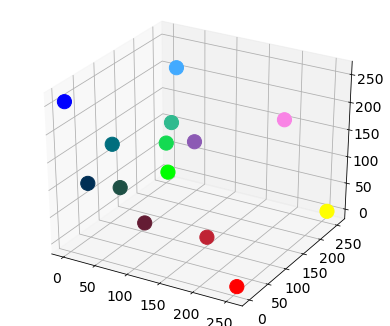
\includegraphics[width = 0.4\textwidth]{3Dcolors.png}}
	\end{figure} 
\end{center}

Попробуем теперь перевести их в 2-мерное пространство. Подберем гиперпараметры:
\begin{itemize}
	\item \verb|metric| --- признаки объектов заданы в числовом виде $\Rightarrow$ можно использовать евклидову метрику $\Rightarrow$ \verb|metric="euclidean"| (по умолчанию)
	\item \verb|n_components| --- мы хотим получить двумерное пространство $\Rightarrow$ \verb|n_components=2| (по умолчанию)
	\item \verb|min_dist| --- посмотрим на разные варианты, чтобы посмотреть и локальную, и глобальную структуру данных: $\{0.1, 0.3, 0.6, 1.0\}$
	\item \verb|n_neighbors| --- сложно подобрать данный гиперпараметр сразу, рассмотрим несколько вариантов: $\{2, 3, 8\}$
\end{itemize}

Для данной выборки не нужна предварительная обработка, поскольку все признаки определяют одну и ту же величину --- интенсивность цвета.
Запустим UMAP и посмотрим на результаты. Уберем оси, так как они показывают лишь значение некоторых абстрактных признаков, которые подобрал UMAP и не дают никакой полезной информации:
\begin{center}
\begin{tabular}{c|c|c|c}
\arrayrulecolor[rgb]{0.8,0.85,1}
	& \verb|n_neighbors=2| & \verb|n_neighbors=3| & \verb|n_neighbors=8| \\
	\hline
	\begin{sideways} \verb|min_dist=0.1| \end{sideways} & \includegraphics*[width = 0.18\textwidth]{0,1colors2.png} & \includegraphics*[width = 0.18\textwidth]{0,1colors3.png} & \includegraphics*[width = 0.18\textwidth]{0,1colors8.png} \\
	\hline
	\begin{sideways} \verb|min_dist=0.3| \end{sideways} & \includegraphics*[width = 0.18\textwidth]{0,3colors2.png} & \includegraphics*[width = 0.18\textwidth]{0,3colors3.png} & \includegraphics*[width = 0.18\textwidth]{0,3colors8.png} \\
	\hline
	\begin{sideways} \verb|min_dist=0.6| \end{sideways} & \includegraphics*[width = 0.18\textwidth]{0,6colors2.png} & \includegraphics*[width = 0.18\textwidth]{0,6colors3.png} & \includegraphics*[width = 0.18\textwidth]{0,6colors8.png} \\
	\hline
	\begin{sideways} \verb|min_dist=1.0| \end{sideways} & \includegraphics*[width = 0.18\textwidth]{1,0colors2.png} & \includegraphics*[width = 0.18\textwidth]{1,0colors3.png} & \includegraphics*[width = 0.18\textwidth]{1,0colors8.png} \\
\end{tabular}
\end{center}

При \verb|n_neighbors=2| четко видно деление цветов на разные кластера. При этом цвета примерно правильно распределились по оттенкам. Здесь UMAP учитывал связи только с ближайшими двумя соседями: искал похожих и ставил их рядом. Поэтому в кластерах примерно по три точки --- они все ближайшие соседи друг друга.

При \verb|n_neighbors=3| кластера начинают сливаться.  Если взять отдельный кластер из предыдущего случая, то теперь к нему присоединяются третьи по счету соседи тех объектов, которые в нем лежали, а за ними ближайшие соседи соседей. Поэтому здесь больше точек в кластерах при \verb|min_dist=0.1| и \verb|min_dist=0.3| и нет явных кластеров при \verb|min_dist>0.3| Но видны сходства с предыдущим относительным положением точек: зеленые лежат рядом друг с другом, темные точки по-прежнему близко.

При \verb|n_neighbors=8| сеть связей еще сильнее. Теперь можно разглядеть глобальную структуру и увидеть плавные переходы оттенков цветов, что напоминает цветовой спектр.

В целом, все три случая похожи на исходное трехмерное пространство. Точки, которые лежали рядом, по-прежнему являются соседями. При \verb|n_neighbors=2| они даже разбиваются на группы, которые можно также увидеть и в исходном пространстве, но менее явно. То есть UMAP также позволяет выполнить небольшой анализ --- он показывает нам взаимосвязи, которые мы не видели на исходных данных.

	\subsection{Для временных рядов}
	\graphicspath{{chapters/time-series/}}
Попробуем сделать то же самое, но для временных рядов. Здесь:
\begin{itemize}
	\item \textbf{Объект} --- переменная, которая меняется с течением времени
	\item \textbf{Признак} --- даты
	\item \textbf{Значение признака} --- значение переменной на конкретную дату
\end{itemize}

На Kaggle есть \href{https://www.kaggle.com/census/advance-retail-sales-time-series-collection}{выборка} по розничным продажам в различных индустриях (еда, одежда, техника и др.) в США. В ней имеются данные об объемах продаж на первое число каждого месяца, начиная с января 1992 года. Воспользуемся данной выборкой для обработки временных рядов на UMAP.

В исходных данных представлено много отраслей. Оставим только девять из них, чтобы посмотреть, как работает алгоритм. Изначально данные находятся в разных файлах --- соединим их в одну выборку.

Теперь в выборке девять объектов, представленных отраслями, но при этом 326 признаков, выраженных в количестве месяцев. То есть нам предстоит перевести 326-мерное пространство в двумерное.

Подберем гиперпараметры:
\begin{itemize}
	\item \verb|metric| --- вновь признаки объектов заданы в числовом виде $\Rightarrow$ можно использовать евклидову метрику $\Rightarrow$ \verb|metric="euclidean"| (по умолчанию)
	\item \verb|n_components| --- посмотрим на двумерное пространство $\Rightarrow$ \verb|n_components=2| (по умолчанию)
	\item \verb|min_dist| --- возьмем несколько значений \verb|min_dist|: $\{0.1, 0.3, 0.6, 1.0\}$
	\item \verb|n_neighbors| --- снова рассмотрим несколько вариантов: $\{2, 4, 5, 9\}$
\end{itemize}

Перед тем, как запускать алгоритм, необходимо обработать выборку. Данные в ней разнообразны, так как определяют продажи в разных отраслях --- соответственно, в каждой отрасли есть свой средним объем продаж, своя дисперсия. Стандартизируем выборку, что можно сделать с помощью \verb|StandardScaler| из \verb|sklearn.preprocessing|.

\newpage
Теперь можно запустить UMAP. Посмотрим, что получается:

\begin{tabular}{c|c|c|c|c}
\arrayrulecolor[rgb]{0.8,0.85,1}
	 & \verb|n_neighbors=2| & \verb|n_neighbors=3| & \verb|n_neighbors=5| & \verb|n_neighbors=7| \\
	 \hline
	 \begin{sideways} \verb|min_dist=0.1| \end{sideways} & \includegraphics*[width = 0.19\textwidth]{min=0,1,n=2.png} & \includegraphics*[width = 0.19\textwidth]{min=0,1,n=3.png} & \includegraphics*[width = 0.19\textwidth]{min=0,1,n=5.png} & 
	 \includegraphics*[width = 0.19\textwidth]{min=0,1,n=7.png} \\
	 \hline
	 \begin{sideways} \verb|min_dist=0.3| \end{sideways} & \includegraphics*[width = 0.19\textwidth]{min=0,3,n=2.png} & \includegraphics*[width = 0.19\textwidth]{min=0,3,n=3.png} & \includegraphics*[width = 0.19\textwidth]{min=0,3,n=5.png} & 
	 \includegraphics*[width = 0.19\textwidth]{min=0,3,n=7.png} \\
	 \hline
	 \begin{sideways} \verb|min_dist=0.6| \end{sideways} & \includegraphics*[width = 0.19\textwidth]{min=0,6,n=2.png} & \includegraphics*[width = 0.19\textwidth]{min=0,6,n=3.png} & \includegraphics*[width = 0.19\textwidth]{min=0,6,n=5.png} & 
	 \includegraphics*[width = 0.19\textwidth]{min=0,6,n=7.png} \\
	 \hline
	 \begin{sideways} \verb|min_dist=1.0| \end{sideways} & \includegraphics*[width = 0.19\textwidth]{min=1,0,n=2.png} & \includegraphics*[width = 0.19\textwidth]{min=1,0,n=3.png} & \includegraphics*[width = 0.19\textwidth]{min=1,0,n=5.png} & 
	 \includegraphics*[width = 0.19\textwidth]{min=1,0,n=7.png} \\
\end{tabular}
\begin{figure}[H]
	\noindent \centering {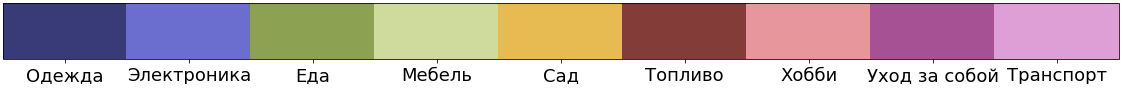
\includegraphics[width =\textwidth]{bar.png}}
\end{figure}

При маленьком значении \verb|n_neighbors| объекты собираются в кластера. Но большие значения \verb|min_dist| увеличивают расстояния между объектами, из-за чего, начиная с трех соседей, кластеры менее заметны.

При \verb|n_neighbors=5| и \verb|n_neighbors=7| кластера незаметны при любом рассмотренном значении \verb|min_dist|. Уже не видно никакой локальной структуры, только общее устройство данных.

Итак, мы получили, что при определенных значениях гиперпараметров объекты группируются в кластера. Теперь поговорим о том, зачем это нужно. В предыдущем примере кластера просто показывали разбиение по оттенкам. Для временных рядов деление на группы означает несколько другое. Кластера временных рядов показывают, какие переменные наиболее похоже по сравнению с остальными меняются во времени.
\newpage
\begin{multicols}{2}
	\fbox{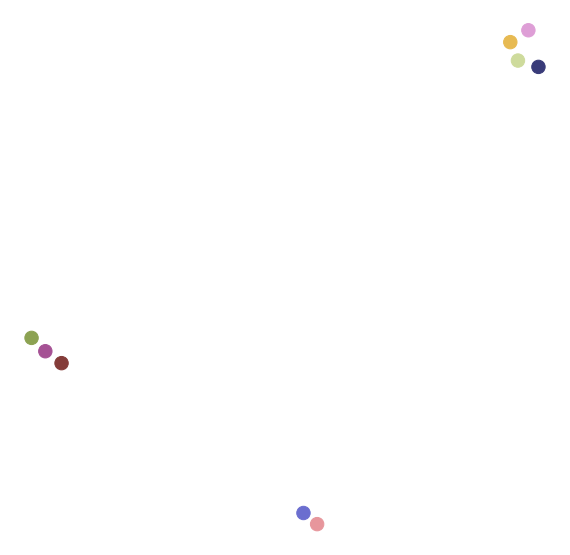
\includegraphics[width=0.9\linewidth]{show.png}\columnbreak}
	
	Рассмотрим изображение, полученное для \verb|n_neighbors=2| и \verb|min_dist=1.0|.
	
	На картинке видно три кластера. Объекты, находящиеся в каждом, похожи между собой. Так, объем розничных продаж электроники и товаров для хобби имеют сходства в траектории движения на протяжении представленных 27 лет. Аналогично можно сказать про топливо, товары для ухода за собой и еду.
	
	Если ряды в одном кластере действительно ведут себя похоже, то корреляция между ними должна быть высокой по сравнению с рядами из другого кластера.
\end{multicols}
\begin{figure}[H]
	\noindent \centering {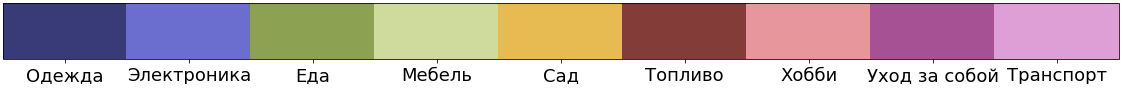
\includegraphics[width=\textwidth]{bar.png}}
\end{figure}

Посчитаем корреляцию между всеми парами объектов:
\begin{figure}[H]
	\noindent \centering {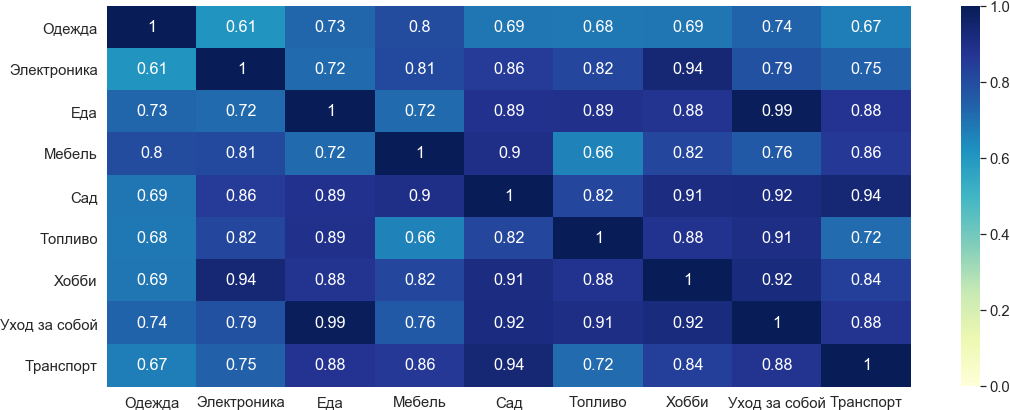
\includegraphics[width =\textwidth]{corr.png}}
\end{figure}

Рассмотрим несколько объектов и ряды, ближайшие к ним по корреляции:
\begin{itemize}
	\item \textbf{Одежда} --- мебель. И действительно, данные два объекта лежат в одном кластере, причем очень близко
	\item \textbf{Электроника} --- хобби. Аналогично, данные два ряда находятся в одном кластере, что показывает их схожесть
	\item \textbf{Мебель} --- сад. Несмотря на то, что ряд <<мебель>> был самым похожим для ряда <<одежда>>, у него самого есть ряд <<сад>> с более высоким коэффициентом корреляции. Таким образом выстраивается цепочка из соседей.
\end{itemize}

Однако UMAP меряет схожесть объектов иначе, чем коэффициент корреляции. Алгоритм учитывает относительное положение объектов, и считает похожими те, между которыми оказалось наименьшее <<расстояние>>, даже если на самом деле они находятся далеко --- просто в представленной выборке не оказалось объектов ближе. Коэффициент корреляции меряет зависимость между объектами, независимо от других объектов.

Построим график, чтобы убедиться в разнице:
\begin{figure}[H]
	\noindent \centering {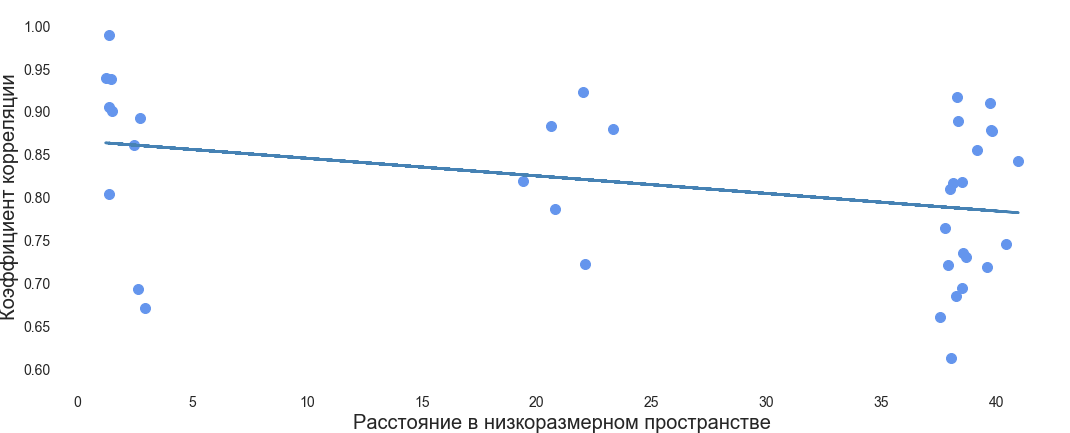
\includegraphics[width =\textwidth]{chart.png}}
\end{figure}

Каждой точке графика соответствует пара рядов. Расстояния между объектами были посчитаны\footnote{Нам не важно само значение расстояния --- нам важно далеко или близко находятся объекты}, исходя из результатов UMAP для \verb|n_neighbors=2|, \verb|min_dist=1.0|. Четкой зависимости между коэффициентом корреляции и расстоянием между объектами нет. Линия тренда показывает слабую отрицательную зависимость, что логично: чем сильнее корреляция, тем больше объекты похожи, тем меньше должно быть расстояние между ними.

Посмотрим также на подобный график для \verb|n_neighbors=7| и \verb|min_dist=1.0|. Увеличение количества соседей создает более глубокую сеть взаимосвязей между объектами, из-за чего учитываются также самые дальние соседи. Это может помочь расширить понятие схожести для UMAP, так как у него будет больше объектов для обучения.
\begin{figure}[H]
	\noindent \centering {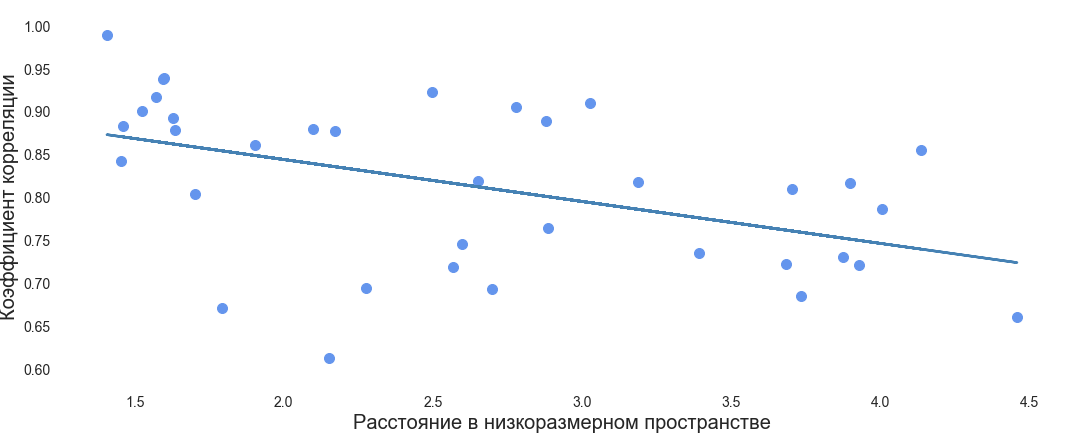
\includegraphics[width =\textwidth]{chart7.png}}
\end{figure} 

Снова линия тренда показывает отрицательную зависимость, но чуть сильнее, чем при \verb|n_neighbors=2|. Разброс точек слишком большой, чтобы говорить о четкой зависимости.

Это подтверждает приведенное ранее утверждение о различиях между данными величинами. Возможно, данная зависимость проявится при большем количестве объектов.

	\newpage
	
	\section{Реализация UMAP}
	\subsection{Выбор данных}
	Для анализа временных рядов был взят \href{https://www.kaggle.com/jessevent/all-crypto-currencies}{датасет}, содержащий информацию о ценах на момент открытия торгов 215 криптовалют в период 2017-2018 годов. Данный датасет был обработан, поэтому в итоговом варианте есть некоторые изменения:
\begin{itemize}
	\item Удалены столбцы с ненужными данными (цены закрытия, спред и др.) --- нам нужны только столбцы с названием, датой и значением цены на момент открытия торгов
	\item Удалена информация о рядах, в данных о которых имеются пропуски --- у некоторых были пропущены даты, соответственно, мы не знаем их значения в данные периоды
	\item Оставлена информация только о рядах, уже существовавших на 1 января 2017 года --- некоторые ряды появлялись позже данной даты, то есть у нас не было информации об их ценах до момента создания данных криптовалют
	\item Удалены данные на ноябрь и декабрь 2018 года --- не у всех выбранных рядов в датасете были указаны цены для данного периода
\end{itemize}


Финальный вариант данных до стандартизации можно найти здесь: *ссылка на репозиторий*
	\subsection{Установка библиотеки}
	Библиотека UMAP требует установки, так как её нет в в стандартном наборе библиотек.

Внутри UMAP также используются библиотеки: \verb|numpy, scipy, scikit-learn, numba| --- они являются обязательными требованиями для успешной установки UMAP. Если вы не уверены, есть ли у вас перечисленные библиотеки, или знаете, что их нет, это не проблема --- при установке они будут добавлены автоматически.

Поставить себе библиотеку UMAP можно следующими способами \cite{umap}:
\begin{itemize}
	\item с помощью \verb|conda: conda install -c conda-forge umap-learn|
	\item с помощью \verb|pip: pip install umap-learn|
	\item ручная установка:
	\begin{enumerate}
		\item Загрузка пакета:\\
		\verb|textwget https://github.com/lmcinnes/umap/archive/master.zip| \\
		\verb|unzip master.zip| \\
		\verb|rm master.zip| \\
		\verb|cd umap-master|
		\item Установка необходимых библиотек:
		\verb|sudo pip install -r requirements.txt|
		\item Установка UMAP:
		\verb|python setup.py install|
	\end{enumerate}
\end{itemize} 




	\subsection{Понижение размерности и визуализация}
	\graphicspath{{main/}}
Как и в примере про временные ряды, нашими объектами изучения являются временные ряды. Подборка рядов по криптовалюте содержит 669 дней (1 января 2017 года --- 31 октября 2018 года), то есть 669 признаков.

Нам предстоит снизить размерность 669-мерного пространства. Применим UMAP:

1. Импортируем необходимые библиотеки:

\begin{minted}{Python}
	import numpy as np # работа с матрицами
	import pandas as pd # работа с наборами данных
	import matplotlib.pyplot as plt # построение графиков
	import umap # алгоритм UMAP
	from sklearn.preprocessing import StandardScaler # стандартизация данных
\end{minted}

2. Загрузим наш набор данных:
\begin{minted}{Python}
	data = pd.read_csv("data.csv")
\end{minted}

3. Стандартизируем выборку, чтобы можно было сравнивать ряды между собой. Используем \verb|StandardScaler| из \verb|sklearn.preprocessing|, о котором мы говорили в примере про временные ряды:
\begin{minted}{Python}
	scaler = StandardScaler()
	data = pd.DataFrame(scaler.fit_transform(data.T)).T
\end{minted}

4. Перед тем как запускать UMAP, подберем гиперпараметры:
\begin{itemize}
	\item \verb|metric="euclidean"| --- аналогично предыдущим примерам, возьмем евклидову метрику, которая подходит для вещественных признаков. Стоит по умолчанию
	\item \verb|n_components=2| --- посмотрим на 2-мерное пространство, чтобы нагляднее увидеть, присутствуют ли кластеры в данных. Стоит по умолчанию
	\item \verb|min_dist| --- вновь возьмем несколько значений: $\{0.01, 0.1, 0.3, 0.6, 1.0\}$
	\item \verb|n_neighbors| --- рассмотрим больше разных вариантов: $\{2, 3, 4, 5, 6, 7, 8, 9, 10, 50, 100\}$, чтобы посмотреть, что проиходит при разных значениях гиперпараметра
\end{itemize}

5. Запустим UMAP для выбранных наборов гиперпараметров. Также зафиксируем $\;$ \verb|random_state|, чтобы сравнивать результаты между собой:
\begin{minted}{Python}
	mindists = [0.01, 0.1, 0.3, 0.6, 1.0]
	neighs = [2, 3, 4, 5, 6, 7, 8, 9, 10, 50, 100]
	embeddings = []
	
	for i in range(len(mindists)):
		for j in range(len(neighs)):
			embedding = umap.UMAP(min_dist=mindists[i],
					      n_neighbors=neighs[j],
					      random_state=1).fit_transform(data)
			embeddings.append(embedding)
\end{minted}

6. Визуализируем результаты:

\begin{tabular}{c|c|c|c|c}
\arrayrulecolor[rgb]{0.8,0.85,1}
	& \verb|n_neighbors=2| & \verb|n_neighbors=3| & \verb|n_neighbors=4| & \verb|n_neighbors=5|\\
	\hline
	\begin{sideways} \verb|min_dist=0.01| \end{sideways} & \includegraphics*[width = 0.2\textwidth]{min=0,01,n=2.png} & \includegraphics*[width = 0.2\textwidth]{min=0,01,n=3.png} & \includegraphics*[width = 0.2\textwidth]{min=0,01,n=4.png} & \includegraphics*[width = 0.2\textwidth]{min=0,01,n=5.png}\\
	\hline
	\begin{sideways} \verb|min_dist=0.1| \end{sideways} & \includegraphics*[width = 0.2\textwidth]{min=0,1,n=2.png} & \includegraphics*[width = 0.2\textwidth]{min=0,1,n=3.png} & \includegraphics*[width = 0.2\textwidth]{min=0,1,n=4.png} & \includegraphics*[width = 0.2\textwidth]{min=0,1,n=5.png}\\
	\hline
	\begin{sideways} \verb|min_dist=0.3| \end{sideways} & \includegraphics*[width = 0.2\textwidth]{min=0,3,n=2.png} & \includegraphics*[width = 0.2\textwidth]{min=0,3,n=3.png} & \includegraphics*[width = 0.2\textwidth]{min=0,3,n=4.png} & \includegraphics*[width = 0.2\textwidth]{min=0,3,n=5.png}\\
	\hline
	\begin{sideways} \verb|min_dist=0.6| \end{sideways} & \includegraphics*[width = 0.2\textwidth]{min=0,6,n=2.png} & \includegraphics*[width = 0.2\textwidth]{min=0,6,n=3.png} & \includegraphics*[width = 0.2\textwidth]{min=0,6,n=4.png}
	& \includegraphics*[width = 0.2\textwidth]{min=0,6,n=5.png}\\
	\hline
	\begin{sideways} \verb|min_dist=1.0| \end{sideways} & \includegraphics*[width = 0.2\textwidth]{min=1,0,n=2.png} & \includegraphics*[width = 0.2\textwidth]{min=1,0,n=3.png} & \includegraphics*[width = 0.2\textwidth]{min=1,0,n=4.png} & \includegraphics*[width = 0.2\textwidth]{min=1,0,n=5.png}\\
\end{tabular}\\[2mm]

При \verb|n_neighbors=2| и \verb|min_dist=0.01| четко видно деление на кластера. С увеличением минимального расстояния между точками кластера все больше размываются, пока почти не сливаются при \verb|min_dist=1.0|.

При \verb|n_neighbors=3| и \verb|min_dist=0.01| заметны кластера, но далее с увеличением \verb|min_dist| они постепенно объединяются.

Далее, начиная с \verb|n_neighbors=4|, при маленьких значениях \verb|min_dist| еще видна локальная структура, но кластера едва заметны --- четко выделяется небольшая группа временных рядов, но в остальном кластера слились воедино. При больших значениях \verb|min_dist| остается только глобальная структура.
\newpage
Рассмотрим оставшиеся варианты \verb|n_neighbors|: $\{6, 7, 8, 9, 10, 50, 100\}$

\begin{tabular}{c|c|c|c|c}
\arrayrulecolor[rgb]{0.8,0.85,1}
	& \verb|n_neighbors=6| & \verb|n_neighbors=7| & \verb|n_neighbors=8| & \verb|n_neighbors=9|\\
	\hline
	\begin{sideways} \verb|min_dist=0.01| \end{sideways} & \includegraphics*[width = 0.2\textwidth]{min=0,01,n=6.png} & \includegraphics*[width = 0.2\textwidth]{min=0,01,n=7.png} & \includegraphics*[width = 0.2\textwidth]{min=0,01,n=8.png} & \includegraphics*[width = 0.2\textwidth]{min=0,01,n=9.png}\\
	\hline
	\begin{sideways} \verb|min_dist=0.1| \end{sideways} & \includegraphics*[width = 0.2\textwidth]{min=0,1,n=6.png} & \includegraphics*[width = 0.2\textwidth]{min=0,1,n=7.png} & \includegraphics*[width = 0.2\textwidth]{min=0,1,n=8.png} & \includegraphics*[width = 0.2\textwidth]{min=0,1,n=9.png}\\
	\hline
	\begin{sideways} \verb|min_dist=0.3| \end{sideways} & \includegraphics*[width = 0.2\textwidth]{min=0,3,n=6.png} & \includegraphics*[width = 0.2\textwidth]{min=0,3,n=7.png} & \includegraphics*[width = 0.2\textwidth]{min=0,3,n=8.png} & \includegraphics*[width = 0.2\textwidth]{min=0,3,n=9.png}\\
	\hline
	\begin{sideways} \verb|min_dist=0.6| \end{sideways} & \includegraphics*[width = 0.2\textwidth]{min=0,6,n=6.png} & \includegraphics*[width = 0.2\textwidth]{min=0,6,n=7.png} & \includegraphics*[width = 0.2\textwidth]{min=0,6,n=8.png}
	& \includegraphics*[width = 0.2\textwidth]{min=0,6,n=9.png}\\
	\hline
	\begin{sideways} \verb|min_dist=1.0| \end{sideways} & \includegraphics*[width = 0.2\textwidth]{min=1,0,n=6.png} & \includegraphics*[width = 0.2\textwidth]{min=1,0,n=7.png} & \includegraphics*[width = 0.2\textwidth]{min=1,0,n=8.png} & \includegraphics*[width = 0.2\textwidth]{min=1,0,n=9.png}\\
\end{tabular}\\[2mm]

Аналогично, для данных значений гиперпараметров уже почти не заметны кластера. Таким образом, с увеличением количества соседей UMAP снижает порог похожести рядов и добавляет в один кластер все менее и менее похожие друг на друга.

\begin{tabular}{c|c|c|c}
\arrayrulecolor[rgb]{0.8,0.85,1}
	& \verb|n_neighbors=10| & \verb|n_neighbors=50| & \verb|n_neighbors=100|\\
	\hline
	\begin{sideways} \verb|min_dist=0.01| \end{sideways} & \includegraphics*[width = 0.27\textwidth]{min=0,01,n=10.png} & \includegraphics*[width = 0.27\textwidth]{min=0,01,n=50.png} & \includegraphics*[width = 0.27\textwidth]{min=0,01,n=100.png}\\
	\hline
	\begin{sideways} \verb|min_dist=0.1| \end{sideways} & \includegraphics*[width = 0.27\textwidth]{min=0,1,n=10.png} & \includegraphics*[width = 0.27\textwidth]{min=0,1,n=50.png} & \includegraphics*[width = 0.27\textwidth]{min=0,1,n=100.png}\\
	\hline
	\begin{sideways} \verb|min_dist=0.3| \end{sideways} & \includegraphics*[width = 0.27\textwidth]{min=0,3,n=10.png} & \includegraphics*[width = 0.27\textwidth]{min=0,3,n=50.png} & \includegraphics*[width = 0.27\textwidth]{min=0,3,n=100.png}\\
	\hline
	\begin{sideways} \verb|min_dist=0.6| \end{sideways} & \includegraphics*[width = 0.27\textwidth]{min=0,6,n=10.png} & \includegraphics*[width = 0.27\textwidth]{min=0,6,n=50.png} & \includegraphics*[width = 0.27\textwidth]{min=0,6,n=100.png}\\
	\hline
	\begin{sideways} \verb|min_dist=1.0| \end{sideways} & \includegraphics*[width = 0.27\textwidth]{min=1,0,n=10.png} & \includegraphics*[width = 0.27\textwidth]{min=1,0,n=50.png} & \includegraphics*[width = 0.27\textwidth]{min=1,0,n=100.png}\\
\end{tabular}\\[2mm]

В итоге, при больших значениях \verb|n_neighbors| получается один кластер, содержащий в себе все ряды, так как UMAP объединяет их в единую структуру через общих соседей.
	\newpage
	
	\section{Анализ результатов}
	\graphicspath{{chapters/cryptocurrency/}}
При разных значениях гиперпараметров получаются разные отображения исходного пространства.

\begin{multicols}{2}
	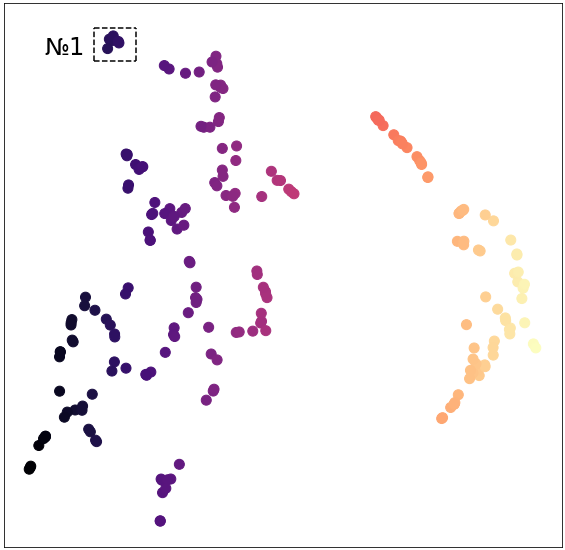
\includegraphics[width=0.85\linewidth]{show.png}\columnbreak
	
	Рассмотрим подробнее результат при \verb|n_neighbors=3| и \verb|min_dist=0.01|. Здесь UMAP рассматривает связь с тремя ближайшими соседями, что позволяет проследить более глубокие взаимосвязи, чем при \verb|n_neighbors=2|. При этом все еще можно различать кластера, то есть можно определить связаны между собой конкретные криптовалюты или нет.
	
	Рассмотрим кластер №1. Исходя из значений двух новых признаков, в данный кластер входят временные ряды: AnarchistsPrime, Einsteinium, GoldBlocks, MonaCoin, TransferCoin, Vertcoin.
\end{multicols}

То есть цены на момент открытия торгов данных криптовалют ведут себя наиболее похоже во времени. Посмотрим на графики цен криптовалют:

\begin{figure}[H]
	\noindent \centering {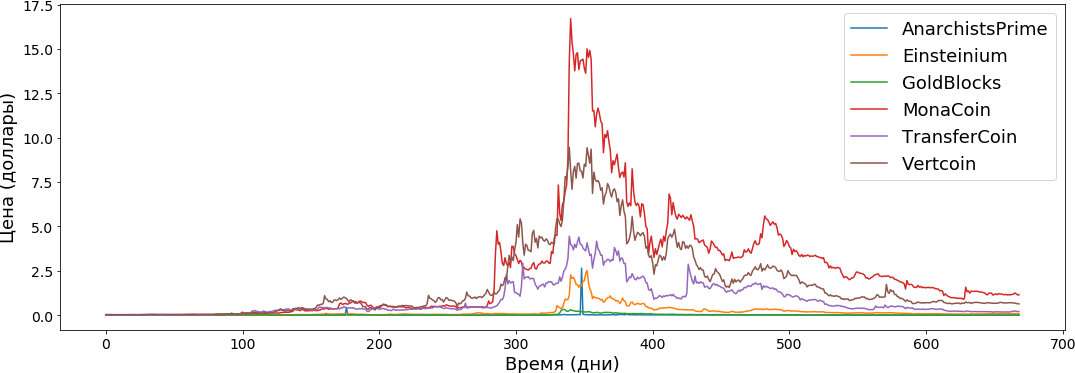
\includegraphics[width = \textwidth]{vecs.png}}
\end{figure}

В самом деле, данные временные ряды имеют похожую динамику. Учитывая стандартизацию данных, они выглядят вот так:

\begin{figure}[H]
	\noindent \centering {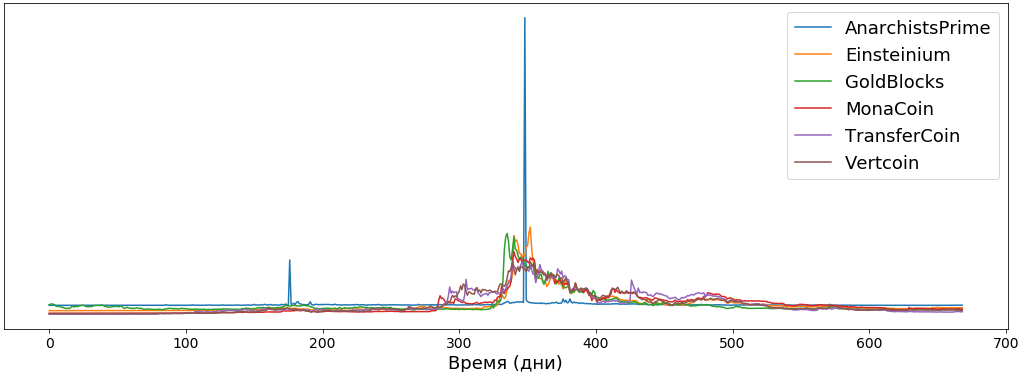
\includegraphics[width = \textwidth]{vecs_s.png}}
\end{figure}

Графики цен криптовалют почти совпадают --- UMAP нашел наиболее похожие ряды, они оказались в одном кластере. Видны небольшие расхождения, например, два внезапных взлета цены AnarchistsPrime. Но если посчитать коэффициенты корреляции, то в целом, ряды сильно коррелируют между собой:

\begin{figure}[H]
	\noindent \centering {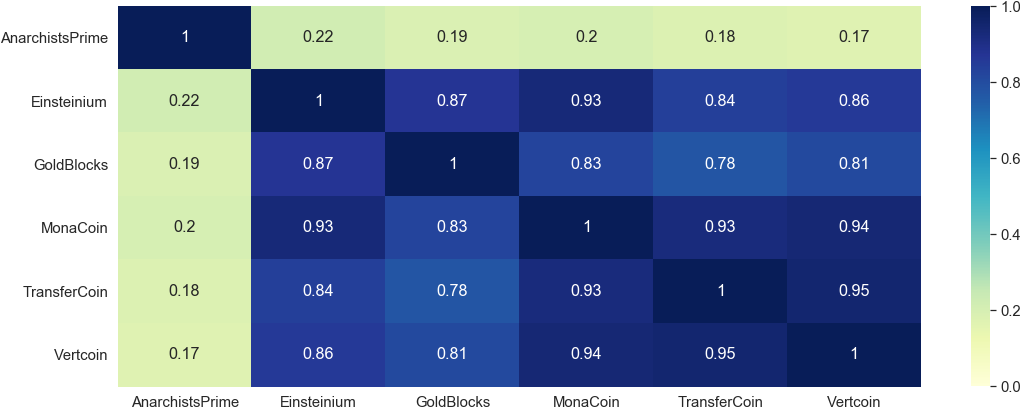
\includegraphics[width = \textwidth]{corr.png}}
\end{figure} 

AnarchistsPrime выбивается из группы криптовалют, имея самые низкие коэффициенты корреляции по сравнению с другими. Как же так получилось, что он оказался в одном кластере с данными рядами?

Ранее мы говорили о том, что расстояния в UMAP и коэффициент корреляции по-разному оценивают схожесть рядов. В этом случае так и вышло. Посчитаем корреляцию между AnarchistsPrime и остальными криптовалютами и найдем наибольший коэффициент:

\begin{figure}[H]
	\noindent \centering {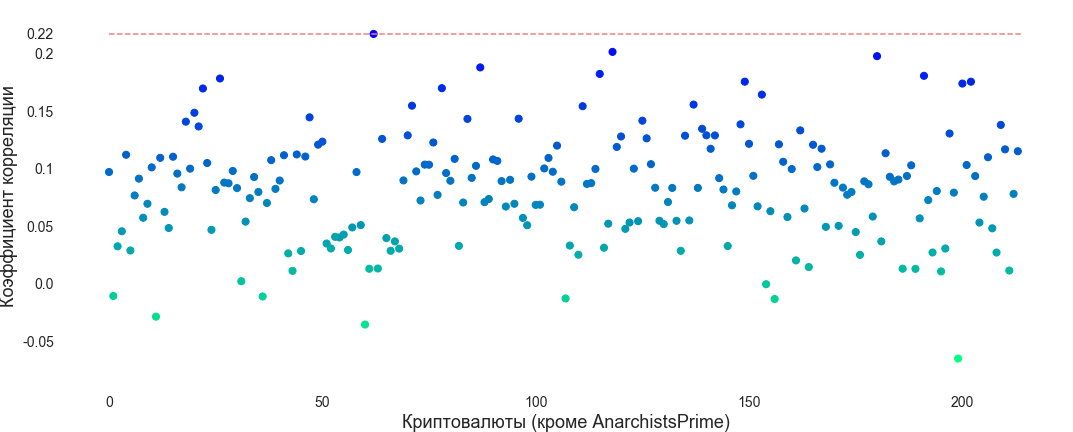
\includegraphics[width = \textwidth]{anarchy.png}}
\end{figure} 

Наибольший коэффициент корреляции временного ряда AnarchistsPrime с другими принимает значение $0.22$ --- корреляция с временным рядом Einsteinium. То есть изменения цены Einsteinium оказались наиболее похожи на поведение AnarchistsPrime, поэтому они оказались в одном кластере. Следующие по схожести ряды также находятся с ним в кластере и имеют чуть меньшие коэффициенты корреляции.
\newpage
\begin{multicols}{2}
	\fbox{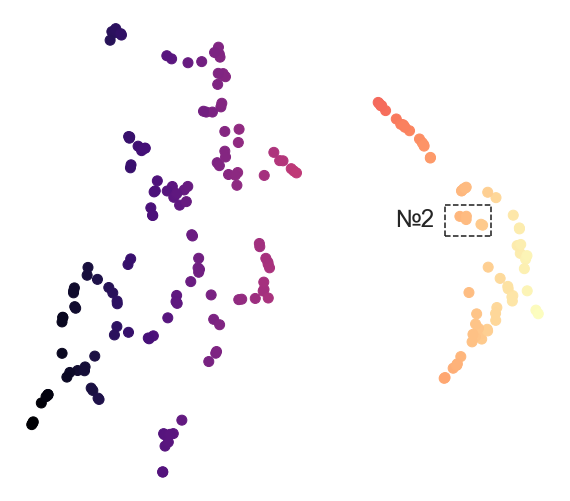
\includegraphics[width=0.85\linewidth]{showy.png}\columnbreak}
	
	Можно также рассмотреть еще один кластер --- желтый (№2). В него входят пять рядов: Augur, Bullion, Decred, Ethereum, Unobtanium.
\end{multicols}

Посмотрим на их графики:

\begin{figure}[H]
	\noindent \centering {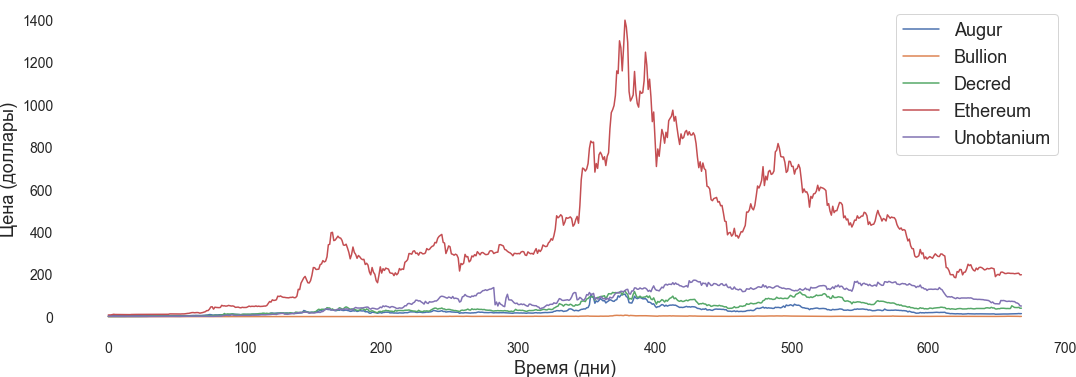
\includegraphics[width = \textwidth]{nvecs.png}}
\end{figure}

Из-за сильной разницы в ценах, особенно с Ethereum, сложно увидеть похожее поведение временных рядов. Построим график со стандартизированными ценами:

\begin{figure}[H]
	\noindent \centering {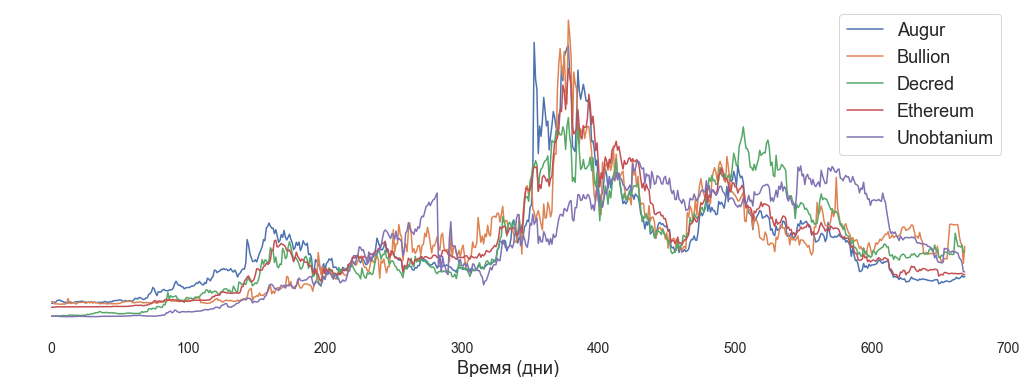
\includegraphics[width = \textwidth]{nvecs_s.png}}
\end{figure}
\newpage
Несмотря на небольшие расхождения, видно, что во многом колебания цен совпадают --- графики накладываются друг на друга. И коэффициенты корреляции принимают большие значения:

\begin{figure}[H]
	\noindent \centering {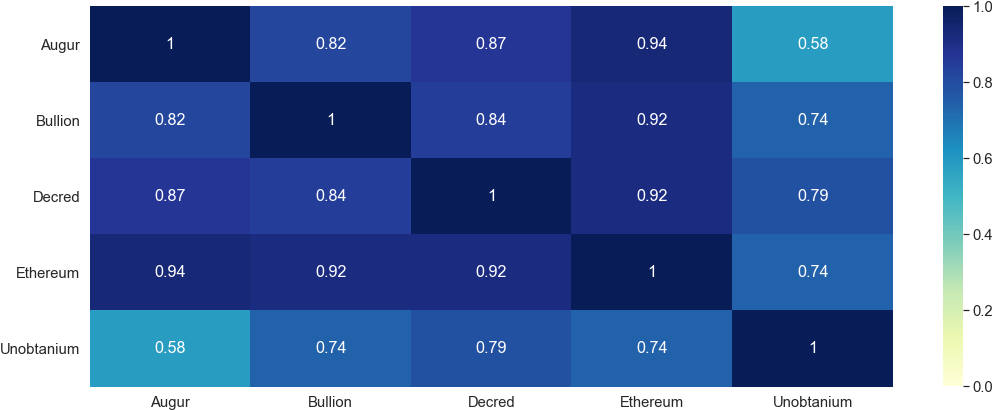
\includegraphics[width = \textwidth]{ncorr.png}}
\end{figure} 

В кластере №2 по сравнению с кластером №1 коэффициенты корреляции не так сильно расходятся во мнении относительно схожести рядов с расстояниями в UMAP.

Мы рассматривали объекты в одном кластере, коэффициенты корреляции между ними принимали большие значения. Но что происходит с объектами, коэффициент корреляции между которыми отрицательный?

Найдем наименьшее значение коэффициента корреляции между рядами. Ему соответствуют ряды AurumCoin и NuBits. Коэффициент корреляции между ними примерно равен $-0.71$. Найдем их на нашей картинке:

\begin{multicols}{2}
	\fbox{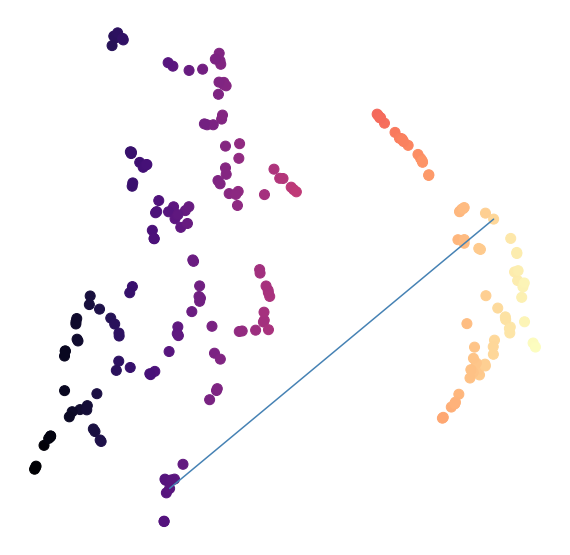
\includegraphics[width=0.85\linewidth]{noncor.png}\columnbreak}
	
	Объекты находятся далеко друг от друга, но некоторые точки лежат на еще большем расстоянии друг от друга. Поскольку изображение, которое мы рассматриваем, было построено для трех ближайших соседей, то UMAP вовсе не учитывал, где будут лежать объекты, являющиеся самыми дальними соседями от исследуемого объекта (для UMAP они даже не являются соседями) --- они отдалились за счет того, что не имеют общих соседей.
\end{multicols}
\newpage
В примере с небольшим количеством рядов мы показали, что коэффициент корреляции отличается от расстояний в UMAP. Посмотрим, что происходит при большом количестве объектов:

\begin{figure}[H]
	\noindent \centering {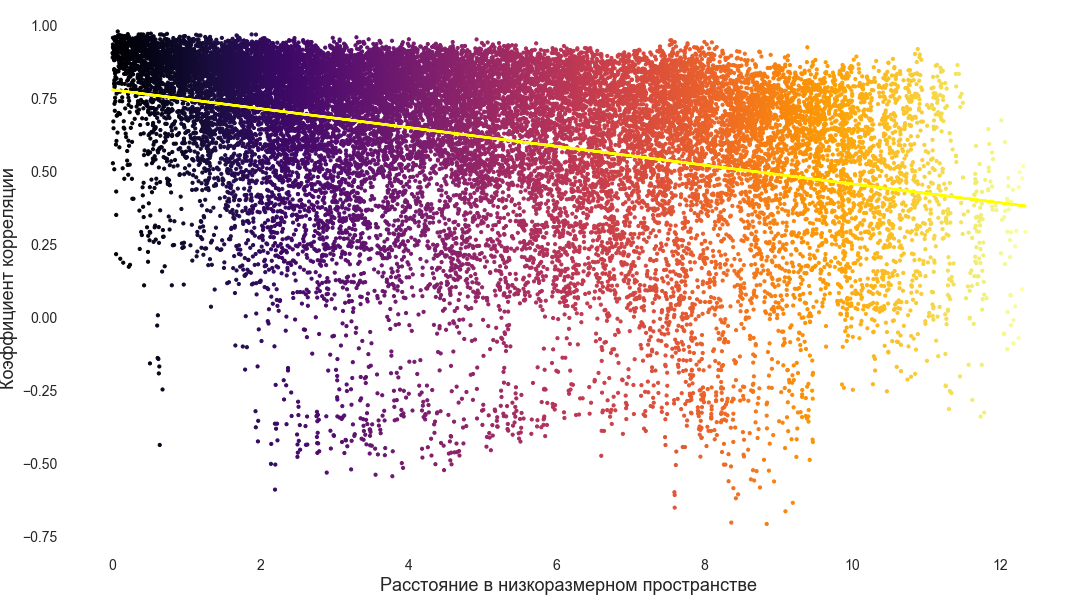
\includegraphics[width = \textwidth]{chart.png}}
\end{figure}

Вновь не видно явной зависимости между коэффициентом корреляции и расстояниями в UMAP --- можно заметить лишь, что при большом коэффициенте корреляции и маленьком расстоянии плотность точек больше, чем в обратной ситуации.

При этом линия тренда имеет отрицательный наклон, как и раньше. И это можно объяснить: UMAP учитывает схожесть тех рядов, которые имеются в выборке, и если совпадает так, что ряды действительно сильно коррелируют, то считает их похожими. Корреляция же измеряет схожесть независимо от других рядов. Поэтому чем больше корреляция, тем меньше расстояние между объектами (потому что они похожи). Но это не работает в обратную сторону: маленькое расстояние между объектами не говорит о сильной корреляции между ними.

Итак, снижение размерности с помощью UMAP и визуализация результатов позволяет взглянуть на внутренние закономерности, существующие в данных.
	\newpage
	
	\section{Заключение}
	Принцип работы алгоритма основывается на построении взвешенного графа в многомерном пространстве, а затем создании его аналога в низкоразмерном. Задача минимизации кросс-энтропии помогает приблизить новый граф к исходному.

Реализация алгоритма, основанная на методе ближайших соседей, позволяет не учитывать взаимосвязи между непохожими объектами и, соответственно, уменьшить время обработки данных, что дает UMAP значительное преимущество в скорости.

В то же время из-за того, что данный метод отбрасывает ненужные связи, при малом количестве соседей даже не похожие объекты могут оказаться ближе, чем похожие. Поэтому необходимо грамотно подбирать основной гиперпараметр алгоритма --- \verb|n_neighbors|. По этой же причине при анализе результатов стоит помнить о том, что алгоритм меряет схожесть, а не отличие --- можно делать выводы только о схожести объектов. Также стоит помнить о разнице между корреляцией и схожести в понятиях UMAP. 

Но несмотря на перечисленные ограничения, использование UMAP может быть очень полезно при анализе любого типа данных. Его применение позволяет снизить размерность исходной выборки, посмотреть на их внутреннее устройство и отследить некоторые закономерности.
	\newpage
	
	\begin{thebibliography}{99}
		\bibitem{reducebasics}
		\href{http://citeseerx.ist.psu.edu/viewdoc/download?doi=10.1.1.98.1478&rep=rep1&type=pdf}{Dimension Reduction | P'adraig Cunningham | Technical Report UCD-CSI-2007-7 | 2007 | 1-2 pages}
		\bibitem{entropy}
		\href{http://colah.github.io/posts/2015-09-Visual-Information/}{Visual Information Theory| Christopher Olah | 2015 }
		\bibitem{mcinnes}
		\href{https://arxiv.org/pdf/1802.03426.pdf}{UMAP: Uniform Manifold Approximation and Projection for Dimension Reduction | Leland McInnes, John Healy, James Melville | 2018 | 13, 17, 26-34 pages}
		\bibitem{hansen}
		\href{https://umap-learn.readthedocs.io/en/latest/api.html}{UMAP | Jakob Hansen | 2018}
		\bibitem{umap}
		\href{https://umap-learn.readthedocs.io/en/latest/how_umap_works.html}{https://umap-learn.readthedocs.io/en/latest/ | UMAP-learn | Main \& How UMAP Works \& Basic UMAP Parameters}
		\bibitem{data}
		\href{https://www.kaggle.com/census/advance-retail-sales-time-series-collection}{Kaggle: Advance Retail Sales Time Series Collection}
		\bibitem{maindata}
		\href{https://www.kaggle.com/jessevent/all-crypto-currencies}{Kaggle: Every Cryptocurrency Daily Market Price}
	\end{thebibliography}
\end{document}